\documentclass{standalone}
\usepackage{tikz}
\usetikzlibrary{patterns, positioning}
\usepackage[sfdefault]{ClearSans} %% option 'sfdefault' activates Clear Sans as the default text font
\usepackage[T1]{fontenc}

\begin{document}
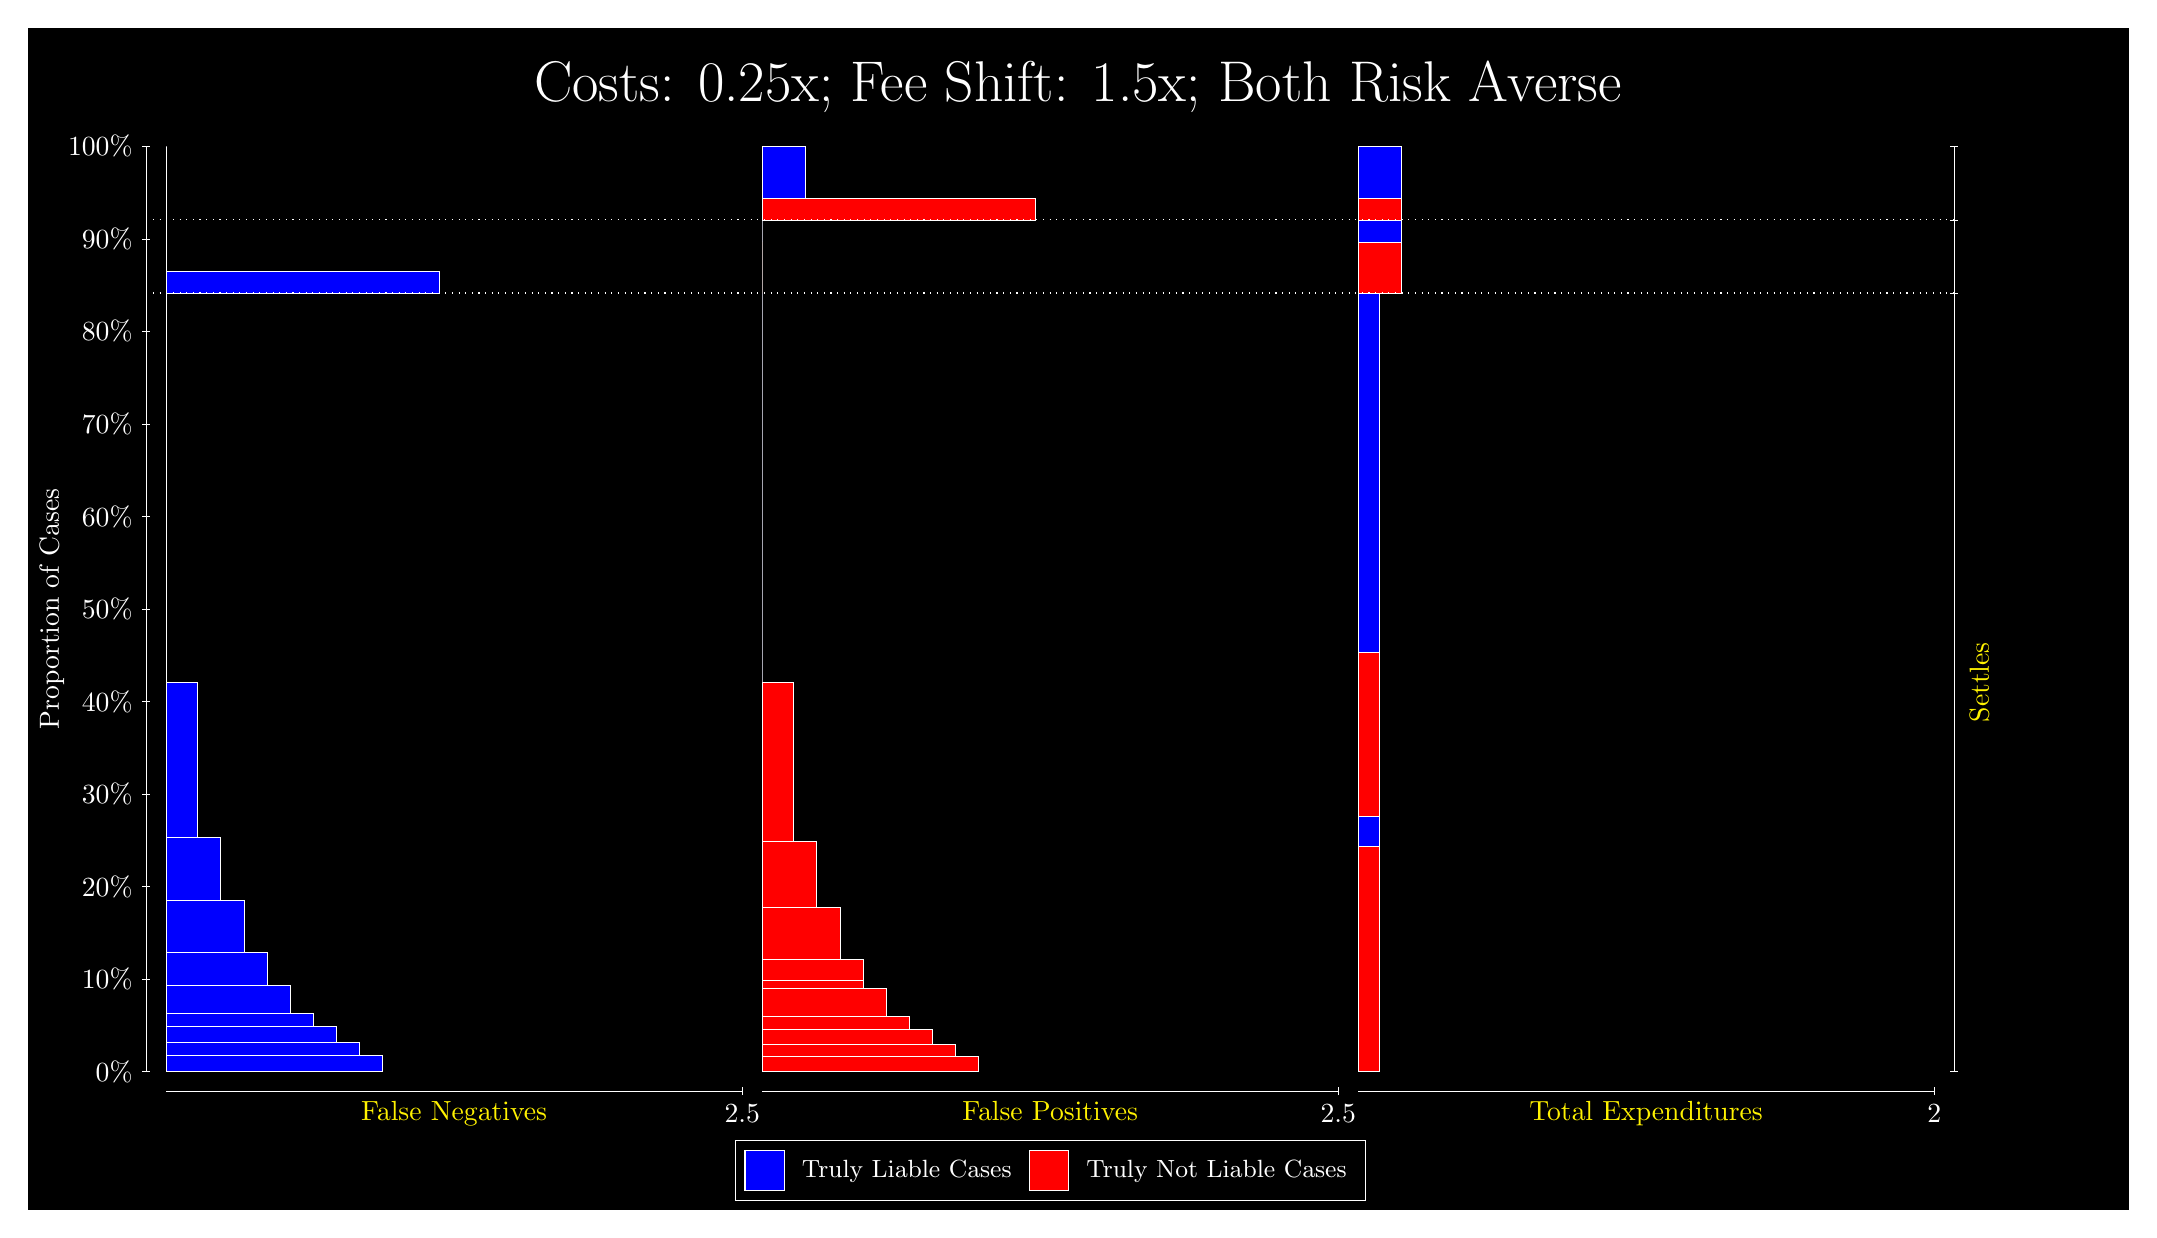
\begin{tikzpicture}
\draw[fill=black] (0,0) rectangle (26.667,15);
\draw[text=white] (0,13.5) rectangle (26.667,15) node[midway] {\huge Costs: 0.25x; Fee Shift: 1.5x; Both Risk Averse};
\draw[white, very thin] (1.5,1.75) -- (1.5,13.5);
\node[rotate=90, text=white, anchor=center] at (0.3, 7.625) {Proportion of Cases};
\draw[white, very thin] (1.45,1.75) -- (1.55,1.75);
\node[text=white, anchor=east] at (1.45, 1.75) {0\%};
\draw[white, very thin] (1.45,2.925) -- (1.55,2.925);
\node[text=white, anchor=east] at (1.45, 2.925) {10\%};
\draw[white, very thin] (1.45,4.1) -- (1.55,4.1);
\node[text=white, anchor=east] at (1.45, 4.1) {20\%};
\draw[white, very thin] (1.45,5.275) -- (1.55,5.275);
\node[text=white, anchor=east] at (1.45, 5.275) {30\%};
\draw[white, very thin] (1.45,6.45) -- (1.55,6.45);
\node[text=white, anchor=east] at (1.45, 6.45) {40\%};
\draw[white, very thin] (1.45,7.625) -- (1.55,7.625);
\node[text=white, anchor=east] at (1.45, 7.625) {50\%};
\draw[white, very thin] (1.45,8.8) -- (1.55,8.8);
\node[text=white, anchor=east] at (1.45, 8.8) {60\%};
\draw[white, very thin] (1.45,9.975) -- (1.55,9.975);
\node[text=white, anchor=east] at (1.45, 9.975) {70\%};
\draw[white, very thin] (1.45,11.15) -- (1.55,11.15);
\node[text=white, anchor=east] at (1.45, 11.15) {80\%};
\draw[white, very thin] (1.45,12.325) -- (1.55,12.325);
\node[text=white, anchor=east] at (1.45, 12.325) {90\%};
\draw[white, very thin] (1.45,13.5) -- (1.55,13.5);
\node[text=white, anchor=east] at (1.45, 13.5) {100\%};

\draw[white, very thin] (24.457,1.75) -- (24.457,13.5);
\draw[white, very thin] (24.407,1.75) -- (24.507,1.75);
\node[anchor=west] at (24.407, 1.75) {};
\draw[white, very thin] (24.407,11.637) -- (24.507,11.637);
\node[anchor=west] at (24.407, 11.637) {};
\draw[white, very thin] (24.407,12.566) -- (24.507,12.566);
\node[anchor=west] at (24.407, 12.566) {};
\draw[white, very thin] (24.407,13.5) -- (24.507,13.5);
\node[anchor=west] at (24.407, 13.5) {};

\draw[white, very thin, fill=blue] (1.75,1.75) rectangle (4.4946,1.953);
\draw[white, very thin, fill=blue] (1.75,1.953) rectangle (4.2018,2.1238);
\draw[white, very thin, fill=blue] (1.75,2.1238) rectangle (3.9091,2.3275);
\draw[white, very thin, fill=blue] (1.75,2.3275) rectangle (3.6163,2.4892);
\draw[white, very thin, fill=blue] (1.75,2.4892) rectangle (3.3236,2.8479);
\draw[white, very thin, fill=blue] (1.75,2.8479) rectangle (3.0308,3.2582);
\draw[white, very thin, fill=blue] (1.75,3.2582) rectangle (2.738,3.9209);
\draw[white, very thin, fill=blue] (1.75,3.9209) rectangle (2.4453,4.7225);
\draw[white, very thin, fill=blue] (1.75,4.7225) rectangle (2.1525,6.6908);
\draw[white, very thin, fill=red] (1.75,6.6908) rectangle (1.75,11.637);
\draw[white, very thin, fill=blue] (1.75,11.637) rectangle (5.2265,11.917);
\draw[white, very thin, fill=red] (1.75,11.917) rectangle (1.75,12.566);
\draw[white, very thin, fill=red] (1.75,12.566) rectangle (1.75,12.846);
\draw[white, very thin, fill=blue] (1.75,12.846) rectangle (1.75,13.5);
\draw[white, very thin, fill=red] (9.3189,1.75) rectangle (12.063,1.9438);
\draw[white, very thin, fill=red] (9.3189,1.9438) rectangle (11.771,2.1);
\draw[white, very thin, fill=red] (9.3189,2.1) rectangle (11.478,2.2858);
\draw[white, very thin, fill=red] (9.3189,2.2858) rectangle (11.185,2.4569);
\draw[white, very thin, fill=red] (9.3189,2.4569) rectangle (10.892,2.8133);
\draw[white, very thin, fill=red] (9.3189,2.8133) rectangle (10.6,2.9032);
\draw[white, very thin, fill=red] (9.3189,2.9032) rectangle (10.6,3.1813);
\draw[white, very thin, fill=red] (9.3189,3.1813) rectangle (10.307,3.8317);
\draw[white, very thin, fill=red] (9.3189,3.8317) rectangle (10.014,4.6701);
\draw[white, very thin, fill=red] (9.3189,4.6701) rectangle (9.7214,6.6965);
\draw[white, very thin, fill=blue] (9.3189,6.6965) rectangle (9.3189,11.637);
\draw[white, very thin, fill=red] (9.3189,11.637) rectangle (9.3189,12.286);
\draw[white, very thin, fill=blue] (9.3189,12.286) rectangle (9.3189,12.566);
\draw[white, very thin, fill=red] (9.3189,12.566) rectangle (12.795,12.846);
\draw[white, very thin, fill=blue] (9.3189,12.846) rectangle (9.8678,13.5);
\draw[white, very thin, fill=red] (16.888,1.75) rectangle (17.162,4.6148);
\draw[white, very thin, fill=blue] (16.888,4.6148) rectangle (17.162,4.9886);
\draw[white, very thin, fill=red] (16.888,4.9886) rectangle (17.162,7.0703);
\draw[white, very thin, fill=blue] (16.888,7.0703) rectangle (17.162,11.637);
\draw[white, very thin, fill=red] (16.888,11.637) rectangle (17.437,12.286);
\draw[white, very thin, fill=blue] (16.888,12.286) rectangle (17.437,12.566);
\draw[white, very thin, fill=red] (16.888,12.566) rectangle (17.437,12.846);
\draw[white, very thin, fill=blue] (16.888,12.846) rectangle (17.437,13.5);
\draw[white, dotted] (1.5,11.637) -- (24.457,11.637);
\draw[white, dotted] (1.5,12.566) -- (24.457,12.566);
\draw[white, very thin] (1.75,1.5) -- (9.0689,1.5);
\node[text=yellow, anchor=north] at (5.4094, 1.5) {False Negatives};
\draw[white, very thin] (9.0689,1.45) -- (9.0689,1.55);
\node[text=white, anchor=north] at (9.0689, 1.45) {2.5};

\draw[white, very thin] (9.3189,1.5) -- (16.638,1.5);
\node[text=yellow, anchor=north] at (12.978, 1.5) {False Positives};
\draw[white, very thin] (16.638,1.45) -- (16.638,1.55);
\node[text=white, anchor=north] at (16.638, 1.45) {2.5};

\draw[white, very thin] (16.888,1.5) -- (24.207,1.5);
\node[text=yellow, anchor=north] at (20.547, 1.5) {Total Expenditures};
\draw[white, very thin] (24.207,1.45) -- (24.207,1.55);
\node[text=white, anchor=north] at (24.207, 1.45) {2};

\node[text=yellow, centered, rotate=90] at (24.777, 6.6936) {Settles};



\draw (12.978300999999998,1.5) node[draw=none] (baseCoordinate) {};
\begin{scope}[align=center]
        \matrix[scale=0.5, draw=white, below=0.5cm of baseCoordinate, nodes={draw}, column sep=0.1cm]{
            \node[rectangle, draw, minimum width=0.5cm, minimum height=0.5cm, fill=blue] {}; &
            \node[draw=none, font=\small, text=white] (B) {Truly Liable Cases}; &
            \node[rectangle, draw, minimum width=0.5cm, minimum height=0.5cm, fill=red] {}; &
            \node[draw=none, font=\small, text=white] (B) {Truly Not Liable Cases}; \\
            };
\end{scope}

\end{tikzpicture}
\end{document}